\chapter{Background}
\label{Background}
This chapter presents the basic idea of a Classification Tree and reviews issues involved when training CART trees to data. By covering various aspects of tree growth, likely reasons as to why existing approaches to growing oblique trees have not caught on are identified. Section~\ref{ClassificationTrees} revisits the idea of a Classification Tree and Section~\ref{TreeInterpretability} follows with a discussion of issues that affect the interpretability of a tree. Doing so demonstrates why oblique splits are sometimes be better suited for growing interpretable trees. Unfortunately, oblique splits are inherently difficult to use as will be explained in Section~\ref{FindingObliqueSplits}. A list of possible explanations why existing approaches to growing oblique trees have not caught on follow in Section~\ref{PossibleReasonsforStatusQuo}.

\section{Classification Trees}
\label{ClassificationTrees}
\subsection{Natural Origins}
\label{NaturalOrigins}
The idea of tree-based classification appears naturally when considering populations with hierarchical structure and is nothing new. Biologists have long used this idea to help identify organisms, botanists to name plants~\cite{nla.cat-vn178734}~\cite{nla.cat-vn2380672} and doctors to assist medical diagnoses~\cite{609112}~\cite{AnneB.Nattinger04011998}. Tree-based classifiers allow subject specialists to distill expert knowledge into a set of easily understandable and transparent rules for others to follow. Figure~\ref{fig_taxonomy_key_biology_table} shows a simple application of this idea in Biology.
\begin{figure}
\centering
\subfigure[Taxonomic Key for various species of plants.]{
    \label{fig_taxonomy_key_biology_table}
	\includegraphics[width=.47\textwidth]{fig_taxonomy_key_biology_table.eps}
}
\subfigure[Graphical representation of information contained in Taxonomic Key.]{
    \label{fig_taxonomy_key_biology_tree}
	\includegraphics[width=.47\textwidth]{fig_taxonomy_key_biology_tree.ps}
}
\caption{Tree-based classification is a natural way of classifying hierarchical populations and has long been used by practitioners from various fields. A Dichotomous Taxonomic Keys in particular ask a series of questions with \emph{Yes} or \emph{No} answers as shown in Figure~\ref{fig_taxonomy_key_biology_table}. It is easy to follow and each path leads to a class prediction. This information can also be represented by a tree (where left branches by convention denote positive answers).}
\label{fig_taxonomy_key_biology}
\end{figure}
Armed with this Taxonomic Key, anyone can easily identify species of plants specified in the Key. If a plant has shoots and does not flower, it is a Pine Tree. If it shoots and flowers but does not have leaves, it is a Cactus Tree. The information contained in this construct can also be shown graphically by a tree as seen in Figure~\ref{fig_taxonomy_key_biology_tree}.\\

Though a great deal of thought is often needed to create such Taxonomic Keys manually, researchers have sought ways of automating this process to extract information from databases in general. The question they have in mind is as follows,
\begin{quote}
\emph{Can tree-based classifiers be automatically grown to data in such a way that they can be used to accurately predict the class of previously unobserved observations?}
\end{quote}
Working independently, researchers from Computer Science~\cite{Quinlan.86}~\cite{Quinlan.88}~\cite{Quinlan.90} and Applied Statistics~\cite{cart84-2} arrived at similar solutions to this problem. With greater cross-fertilization of ideas and additional input from the Engineering community~\cite{Sethi.Sarvarayudu.82}, Breiman \emph{et al} proposed the widely accepted \emph{Classification and Regression Trees} algorithm in 1984 still widely used today. An overview of these ideas follow.

\subsection{Tree Growth}
\label{TreeGrowth}
Given classification data of the form $\mathcal{T}=\left(C^i,X_1^i,\ldots,X_p^i\right)_{i=1}^N=\left(C^i,\Xb^i\right)_{i=1}^N$, a Classification Tree is grown to it by recursively partitioning observations into smaller subsets where observations have more similar classes. This process is naturally representable as a tree with
\begin{itemize}
\item[-] internal nodes were tests partition observations,
\item[-] branches from nodes which represent the outcomes of these tests and
\item[-] leaves at the bottom\footnote{Trees are conventionally drawn with its root at the top of a page growing downwards.} of the tree.
\end{itemize}
When using Classification Trees for prediction, observations are passed through the tree and classified by the class associated to the leaf where it falls. These ideas are illustrated in Figure~\ref{fig_typical_CART_tree}.
\begin{figure}
\centering
\subfigure[Example of a binary splitting axis-parallel tree.]{
	\label{fig_typical_CART_tree_plot_tree}
	\includegraphics[width=.47\textwidth]{fig_typical_CART_tree_plot_tree.ps}
}
\subfigure[The associated decision boundaries defined by the tree on the feature space.]{
	\label{fig_typical_CART_tree_decision_boundaries}
	\includegraphics[width=.47\textwidth]{fig_typical_CART_tree_decision_boundaries.ps}
}
\caption{The above tree is grown to a training set where observations have two continuous attributes $p=2$ with observations from four classes $C\in\left\{1,\ldots,4\right\}$. Four dichotomous tests are applied at internal nodes to produce five leaves. The classes associated to each leaf are shown at the bottom of a tree. With $p=2$, it is possible to view the associated decision boundaries defined by the tree on the feature space $\Xb=\mathbb{R}^2$. As axis-parallel splits are used to partition observations, the feature space is partitioned with rectangular blocks.}
\label{fig_typical_CART_tree}
\end{figure}
As can be seen, five tests partition observations from four classes and good separation is achieved between observations of each class.\\

Though the idea of a Classification Tree allows arbitrarily complex tests at internal nodes, CART trees focus on univariate binary splits to simplify the problem. Tests are univariate in that only one attribute is used to construct each test and binary in that they result in exactly two outcomes. Trees grown in this manner partition observations into (high-dimensional) rectangular blocks as seen in Figure~\ref{fig_typical_CART_tree_decision_boundaries}.\\

With $p$ attributes in total (of which $q$ are continuous say), many tests can be applied during tree growth at each internal node. The exact form of tests considered by CART trees depends on the type of data it is based on.
\begin{description}
\item[$X_i$ continuous:] tests are constrained to be of the form $X_i<c$ v.s. $X_i\geq c$ for some constant $c\in\mathbb{R}$
\item[$X_i$ categorical:] tests are constrained to be of the form $X_i\in A$ v.s. $X_i\notin A$ for some subset $A$ of the factors of the categorical attribute $\left\{a_1,\ldots,a_{|X_i|}\right\}$ 
\end{description}
Of the numerous tests that exist, the one ``best partitioning observations of each class'' (the best split) is applied and the process repeated on child nodes. An impurity measure to compare tests (somehow quantifying this concept) is used. This is examined in greater detail later on.\\

Having understood the generative process of recursive partitioning, we consider two techniques employed by CART trees to avoid overfitting\footnote{Highly parameterized statistical models can fit training data perfectly (low variance) though will not predict well to previously unobserved observations (high bias); the bias-variance tradeoff~\cite{Geu02}~\cite{citeulike:161814}.}. The first employs the early stopping of recursive partitioning during tree growth and the logic is simple, 
\begin{itemize}
\item[-] if recursive partitioning proceeds until all training set observations are perfectly classified, the tree is like to have focused more on specific occurrences in the training set rather than generalities in the population,
\item[-] recursive partitioning should therefore stop before leaves become pure (observations at each leaf are all of the same class)
\end{itemize}
To achieve this, recursive partitioning terminates at a node if any of the following criteria are satisfied,
\begin{description}
\item[Pure Nodes:] if all observations at a node are of the same class, recursive partitioning terminates (further partitions add no value).
\item[Size Threshold:] if a node contains fewer than some prespecified number of observations (defaulted to 10), recursive partitioning terminates (trees should not focus on small details). 
\item[Impurity Threshold:] if impurity at a node is below some prespecified proportion of that of the entire training set (defaulted to 0.01), recursive partitioning terminates (such nodes are considered to be \emph{sufficiently pure}).
\item[Child Node Threshold:] if applying the best split produces a child node with fewer than some prespecified number of observations (defaulted to 5), recursive partitioning terminates (leaves should not become too specialized).
\end{description}
Unfortunately, early stopping is not sufficient to ensure that resulting CART trees generalize\footnote{A classifier that generalizes is one that is not overfit; it makes good class predictions for previously unobserved observations.}. Breiman \emph{et al} propose the following complementary technique to address this issue.

\subsection{Cost-Complexity Pruning}
\label{CostComplexityPruning}
Growing trees that generalize can be thought of as tackling an optimal stopping problem for the recursive partitioning process (trees should be grown to data to learn from it but they should not be overgrown). When exactly should one stop? \\
%This allows all avenues to be investigation during tree growth and allows a simple generalizing tree to be obtained. \\
%Early stopping prevents trees from focusing on small details, it can also obstructing the discovery of potentially useful splits (recursive partitioning may terminate just as tree growth is onto something).

Cost-complexity pruning avoids this question altogether by simply growing a tree until it is overfit (a maximal tree) and by ``looking backwards from it'' to find rooted subtrees of it that \emph{do} generalize. Instead of considering all possible rooted subtrees\footnote{The number of rooted subtrees of a maximal tree is potentially vast. For binary trees with $l$ leaves, Breiman \emph{et al}~\cite{cart84-2} pg. 284 calculate an upper bound to be $\lfloor 1.5028369^l\rfloor$ with an exact bound in the case of saturated trees (trees with $n$ levels of internal nodes with a full complement of $2^n$ leaves). A 3-levelled saturated tree has $26 = \lfloor (1.5028369)^{2^3}\rfloor$ rooted subtrees while a 4-levelled saturated tree has $677 = \lfloor (1.5028369)^{2^4}\rfloor$. All rooted subtrees of a 3-levelled saturated tree are identified in Figure~\ref{fig_rooted_subtrees}. It is easy to see the multiplicative effect that each internal node has on the total number of rooted subtrees.}\begin{figure}
\centering
\includegraphics[width=1\textwidth]{fig_rooted_subtrees.ps}
\caption{A 3-levelled saturated tree is shown in the top-left plot with its nodes labeled. The other plots show its rooted subtrees, rows 1 to 4 showing those where neither nodes 2 and 3 are absent, row 5 showing those where only node 3 is absent, row 6 showing those where only node 2 is absent and the rest follow on the last row. One sees that the total number of rooted subtrees grows in a multiplicative manner with each additional internal node.}
\label{fig_rooted_subtrees}
\end{figure}, cost-complexity pruning focuses on a specific subset of them found as follows. For trees $T$, let
\begin{description}
\item[$R(T)$] denote a measure of its goodness of fit found by adding contributions $r(t)$ over its leaves $t$ (the number of misclassifications or impurity say) and
\item[$size(T)$] denote a penalty measure that increases as trees become ``more complex'' (the number of leaves say)
\end{description} 
then use the following measure to compare rooted subtrees of a maximal tree $$R_k(T)=R(T)+k~size(T).$$
For any given $k$, $R_k(T)$ weights the ability of a rooted subtree $T$ to fit training data against its complexity allowing comparison of rooted subtrees. Breiman \emph{et al} propose focusing on rooted subtrees that minimize $R_k(T)$ for each value of $k\in\mathbb{R}$. Amazingly, Breiman \emph{et al} show\footnote{Concise version of these proofs are found in Ripley~\cite{Ripley.96}.}~\cite{cart84-2} pg. 284--293 that a nested family of rooted subtrees $\left\{T_i\right\}_{i=0}^K$ is optimal over all $k$ and that each $T_i$ is optimal over some range $k\in[k_i,k_{i+1})$ with $$-\infty=k_0<k_1<\ldots<\infty.$$ In addition to this, they also give a method for finding the $k_i$'s as well as an algorithm to construct the entire tree sequence $\left\{T_i\right\}_{i=0}^K$. The cost-complexity tree that best generalizes is easily identified and used as the final classifier. The entire process is a illustrated in Figure~\ref{fig_tree_pruning}. 
\begin{figure}
\centering
\includegraphics[width=1\textwidth]{fig_tree_pruning.ps}
\caption{Cost-complexity pruning allows trees that generalize well to be found. Starting with a fully grown (and thus overfit tree), a family of rooted subtrees $\left\{T_i\right\}_{i=0}^K$ is easily extracted from it to be used as candidates for the final classifier. Trees in $\left\{T_i\right\}_{i=0}^K$ are nested with increasing $i$ and each $T_i$ minimizes $R_k(T)$ over the range $k\in[k_i,k_{i+1})$. Though prediction error over the training set (in-sample error) increases with $i$, out-of-sample error needed not; the best generalizing tree is used as the final classifier. In the above example, $T_1$ say, might have the lowest out-of-sample prediction error and thus be used as the final classifier.}
\label{fig_tree_pruning}
\end{figure}

\section{Tree Interpretability}
\label{TreeInterpretability}
As mentioned previously, the interpretability of a tree is its main strength. Though each univariate binary split is interpretable in isolation, the interpretability of an entire axis-parallel tree need not be. Tree interpretability deteriorates as trees become larger as seen in Figure~\ref{fig_tree_interpretability}.\\
\begin{figure}
\centering
\includegraphics[width=.49\textwidth]{fig_tree_interpretability_more.ps}
\includegraphics[width=.49\textwidth]{fig_tree_interpretability_less.ps}
\caption{The interpretability of a tree depends on two factors, the interpretability of each split in isolation and its cumulative effect over the entire tree. A balance should be achieved between using simple tests that are easy to understand and more complex tests that allow smaller trees to be grown.}
\label{fig_tree_interpretability}
\end{figure}

The reason why some trees are larger than others simply comes down to the interplay between how observations of different classes are distributed over the feature space and the tests used to partition them; recursive partitioning will proceed until all leaves are sufficiently pure with whatever tests it is allowed to use. One way of obtaining smaller trees is to consider more general splits during tree growth. For tests over continuous attributes, a multivariate generalization of axis-parallel splits is an oblique split $\sum_{i=1}^q a_iX_i<c$ (assuming continuous attributes lie in the first $q$ positions). Oblique splits are better suited to partitioning observations as shown in Figure~\ref{fig_power_of_splits}.\\
\begin{figure}
\centering
\subfigure[A single oblique split is enough to partition observations in this example.]{
	\label{fig_power_of_splits_oblique}
	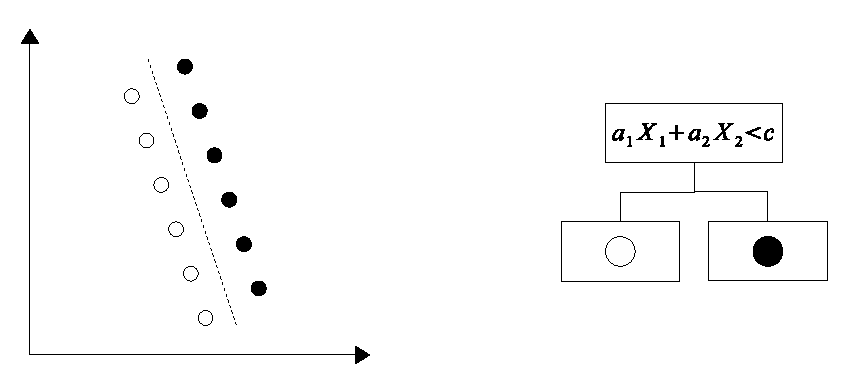
\includegraphics[height=4cm]{fig_power_of_splits_oblique.ps}
}
\subfigure[An axis-parallel tree requires more that one level of splits to achieve the same purity within its leaves as a single oblique split.]{
	\label{fig_power_of_splits_axis_parallel}
	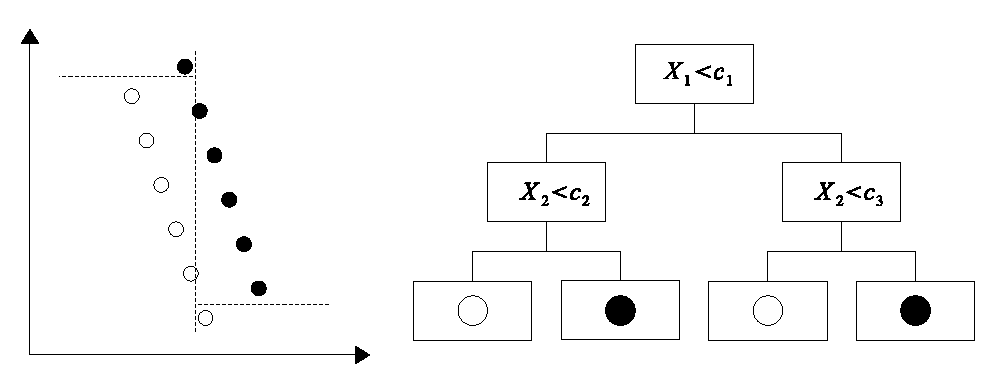
\includegraphics[height=4cm]{fig_power_of_splits_axis_parallel.ps}
}
\caption{Observations from this two-class classification problem are easily partitioned with a single oblique split as shown in Figure~\ref{fig_power_of_splits_oblique}. A single axis-parallel split however cannot produce the same partitioning requiring another level of splits to achieve the same result as shown in Figure~\ref{fig_power_of_splits_axis_parallel}. Oblique splits are better able at partitioning observations so oblique trees should be smaller than axis-parallel trees.}
\label{fig_power_of_splits}
\end{figure}

Though oblique splits naturally result in smaller trees, they are not necessarily more interpretable. In calling oblique splits that use all $q$ continuous attributes full oblique splits, we state the obvious in that full oblique splits are less interpretable than those using fewer attributes, e.g. $X_1>0.25 X_2$ v.s. $X_1>0.25 X_2+0.5 X_3+X_4$. Unwarranted use of full oblique splits to grow oblique trees can paradoxically reduce interpretability as it results in ``cluttered trees'' (the problem becomes more acute with increasing $q$). Though oblique splits may be useful at time, concise oblique splits should always be used \emph{whenever possible} to obtain more interpretable trees.

\section{Finding Oblique Splits}
\label{FindingObliqueSplits}
Putting aside the issue of how one obtains interpretable oblique trees for the meantime, it is instructive to analyze the problem of finding the best full oblique split at each stage of tree growth. One ideally applies the test with the lowest impurity which implies that \emph{all oblique splits} must be considered. By introducing the idea of a split dictionary, it is possible to directly compare the magnitude of the computational problems posed when finding the best oblique split with that of the best axis-parallel split. \\

A split dictionary (for a family of splits) is a set of splits of minimal size that produces all possible partitioning of observations (permitted by that family of splits) over the training set. Figure~\ref{fig_split_dictionaries} shows possible axis-parallel and oblique split dictionaries for a small dataset.
\begin{figure}
\centering
\subfigure[Example of an axis-parallel split dictionary.]{
	\label{fig_split_dictionary_axis_parallel}
	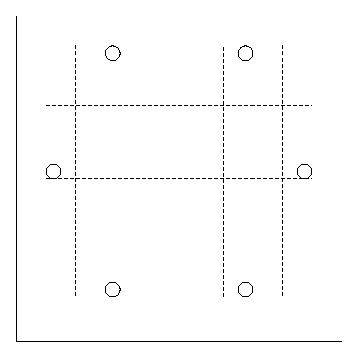
\includegraphics[width=.45\textwidth]{fig_split_dictionary_axis_parallel.eps}
}
\subfigure[Example of an oblique split dictionary.]{
	\label{fig_split_dictionary_oblique}
	\includegraphics[width=.45\textwidth]{fig_split_dictionary_oblique.eps}
}
\caption{
A split dictionary (for a family of splits) is a set of splits of minimal size that produces all possible partitioning of observations (permitted by that family of splits) over the training set. Though split dictionaries need not be unique (small perturbations produce new split dictionaries), its size stays constant for a given dataset. Figure~\ref{fig_split_dictionary_axis_parallel} shows a possible axis-parallel split dictionary for a small dataset and is of size 6. No other partitioning of observations can result with axis-parallel splits other than those generated here. Figure~\ref{fig_split_dictionary_oblique} shows a possible oblique split dictionary for the same data and is of size 15 (it is larger as oblique splits can produce different partitions of the observations).}
\label{fig_split_dictionaries}
\end{figure}
Though there are often many split dictionaries for a family of splits, its size remains constant for a given dataset.\\

We start by considering axis-parallel splits $X_i<c$. For a generic training set $\mathcal{T}$ with $q$ continuous attributes of size $N$, though there may be uncountably many splits ($c\subset B\subseteq\mathbb{R}$), only a finite number of outcomes will ever occur over the training set. If there are $L_i$ unique values of $X_i$ in $\mathcal{T}$, there will therefore be exactly $L_i-1$ unique outcomes over attribute $X_i$. The size of the axis-parallel split dictionary (for all attributes) is therefore $\sum_{i=1}^q (L_i-1)$. With each $L_i$ at most $N$, the axis-parallel split dictionary can be seen to grow at most linearly in both $N$ and $q$.\\

A direct calculation of the size of the oblique split dictionary is very difficult. Fortunately however its size can be shown to be exactly $\left\{2\sum_{k=0}^{q} {L_{gen}-1\choose k}-2\right\}/2$ where $L_{gen}$ is the number of generally positioned\footnote{A set of $q$-dimensional vectors are generally positioned if every subset of size $q$ or less is linearly independent.} $q$-dimensional points in $\mathcal{T}$ and is a consequence of a combinatorial geometry result\footnote{Given $L_{gen}$ generally positioned points in $q$-dimensional space, there are exactly $2\sum_{k=0}^{q-1} {L_{gen}-1\choose k}$ ways of partitioning them into two bins as specified by which side of the hyperplane $\left\{x:w\cdot x=0\right\}$ they fall. Cover (1965) extended this result to enumerate the number of ways there are to partition points with more general hyperplanes of the form $\left\{x:w\cdot \phi(x)=0\right\}$ for general functions $\phi()$. Choosing $\phi(x)=(1,x)$ in particular shows there are exactly $2\sum_{k=0}^{q} {L_{gen}-1\choose k}$ ways of binning points across hyperplanes with arbitrary intercept. This includes the trivial cases where all points are assigned to the same bin and also double counting across bins.} by Cover~\cite{Cover65}. Assuming $L_{gen}$ is similar to $N$ (it can only be much less if all $q$-dimensional observations from the training set lie in a space of much lower dimensionality) shows that the oblique split dictionary grows extremely fast in both $N$ and $q$. \\

As $N$ and $q$ are often large in real-life datasets, it is practically impossible to find the best oblique split at each stage of tree growth. Existing approaches to growing oblique trees avoid this computational explosion in one of two ways,
\begin{itemize}
\item[-] choosing to focus on a subset of the oblique split dictionary
\item[-] searching for the best split while enforcing an early stop
\end{itemize}
A suboptimal oblique split is and can only be used. Further details follow in Chapter~\ref{ExistingWork}.

\section{Possible Reasons for Status Quo}
\label{PossibleReasonsforStatusQuo}
Though much work has been done on growing oblique trees, none of the existing approaches have caught on. Possible reasons as to why this might be are given below.
\begin{description} 
\item[Intellectual Appeal of the Approach:] Existing approaches to growing oblique trees find oblique splits in archaic ways. This does not give confidence to users in the suitability of such approaches. 
\item[Multiplicity of Trees:] To avoid the computational explosion noted in Section~\ref{FindingObliqueSplits}, some approaches find oblique splits stochastically which produces different a tree each time it is run. Though this is not necessarily a problem, no well-defined approach is given as to how one obtains a ``final classifier'' to use from many that can be grown. 
\item[Interpretability of Trees:] Most work is content with simply growing oblique trees with full oblique splits. Full oblique trees are not necessarily interpretable and so have no comparative advantage over other classifiers.
\item[Easily Accessible Implementations:] It is difficult to obtain and apply implementations of these approaches to real data.
\end{description}
%As has been shown in this chapter, it can be difficult to find oblique splits let alone growing an interpretable oblique tree. 
This thesis seeks to address each of these shortcomings by proposing an intellectually appealing approach to growing more interpretable oblique trees while providing an easily accessible implementation of this approach for others to use.